%!TeX program = xelatex
\documentclass[12pt,hyperref,a4paper,UTF8]{ctexart}
\usepackage{SJTUReport}
\usepackage{float}

%%-------------------------------正文开始---------------------------%%
\begin{document}

%%-----------------------封面--------------------%%
\cover

%%------------------摘要-------------%%
%\begin{abstract}
%
%在此填写摘要内容
%
%\end{abstract}

\thispagestyle{empty} % 首页不显示页码

%%--------------------------目录页------------------------%%
\newpage
\tableofcontents

%%------------------------正文页从这里开始-------------------%
\newpage

%%可选择这里也放一个标题
%\begin{center}
%    \title{ \Huge \textbf{{标题}}}
%\end{center}

\section{实验目的}
\begin{itemize}
    \item 掌握乌贝路德(Ubbelohde)黏度计测定黏度的原理和使用方法。
    \item 测定线性高聚物聚乙二醇的黏均相对平均摩尔质量。
\end{itemize}


\section{实验原理}
在高聚物的研究中,摩尔质量是一个重要的基础数据。高聚物摩尔质量的大小对高聚物的性能影响很大,如橡胶的硫化程度,聚苯乙烯和醋酸纤维等薄膜的抗张强度,纺丝黏液的流动性等,均与其有密切关系。但高聚物分子大小不一,参差不齐,摩尔质量数量级一般在$10^3$-$10^7$之间,所以通常所测高聚物的摩尔质量是平均值。

高聚物平均摩尔质量的测定方法很多,对线性高聚物有端基分析、沸点升高、凝固点降低、等温蒸馏、渗透压、光散射和超离心沉降积扩散等分析方法。这些方法除端基分析外,一般都需要较复杂的仪器设备,且操作繁琐。对于同一聚合物,其测得的数均、质均、Z均或黏均摩尔质量在数值上往往不同。渗透压、光散射及超离心沉降平衡等法测得的平均摩尔质量为绝对值。黏度法能测出平均摩尔质量的相对值。黏度法测定高聚物的相对平均摩尔质量,设备简单,操作方便,有较好的实验精度,其适用的相对摩尔质量范围为$10^4$-$10^7$。

高聚物稀溶液的黏度,主要反映了液体在流动时存在的内摩擦,其中溶剂分子之间相互产生的内摩擦表现出的黏度称为纯溶剂黏度,记作$\eta _0$。此外还有高聚物分子间内的摩擦,以及高聚物分子与分子间的内摩擦,三者总和表现为溶液的黏度,记作$\eta$。在同一温度下,高聚物溶液的黏度一般都比纯溶剂的黏度大得多,即$\eta > \eta_0$,相对于溶剂,溶液粘度增加的分数成为\textit{增比黏度},记作$\eta _{sp}$,即
\begin{equation}
    \eta _ {sp} = \frac{\eta - \eta_0}{\eta_0} = \frac{\eta}{\eta _0} -1 = \eta _r -1
\end{equation}


式中的$\eta _r$成为相对黏度,反映的是溶液的黏度行为。而增比黏度$\eta _ {sp}$则反映的是扣除了溶剂分子之间的内摩擦效应,仅留下纯溶剂与高聚物之间以及高聚物分子之间的内摩擦效应。但高聚物溶液浓度越大,黏度也越大,为了便于比较,用单位浓度下的增比黏度即比浓黏度$\frac{\eta _{sp}}{c}$,或比浓对数黏度$\frac{ln \eta_r}{c}$,作为高聚物相对摩尔质量的量度。当溶液无限稀释时,每个高聚物分子彼此相隔极远,其相互间的内摩擦可忽略不计,此时溶液所表现出的黏度主要反映了高聚物分子与溶剂分子间的内摩擦,定义为特性黏度$[\eta]$。其值取决于溶剂的性质及高聚物分子的形态和大小,与浓度无关。

\begin{equation}
    [\eta] = \lim_{c \to 0}\frac{\eta _{sp}}{c} = \lim_{c \to 0}\frac{\eta _{r}}{c}
\end{equation}

在足够稀的高聚物溶液中,$\frac{\eta _{sp}}{c}$与c和$\frac{ln \eta_r}{c}$与c之间的关系可由经验公式表示:
\begin{equation}
    \frac{\eta _{sp}}{c} = [\eta] + k^{'} [\eta]^2 c
\end{equation}
\begin{equation}
    \frac{ln \eta_r}{c} = [\eta] - \beta [\eta]^2 c
\end{equation}
式中:$k^{'}$和$\beta$为比例系数,因此,通过$\frac{\eta _{sp}}{c}$对c和$\frac{ln \eta_r}{c}$对c作图将得到两条直线,外推至c趋于0时所得截距即为$[\eta]$。

\begin{figure}[htp]
    \centering
    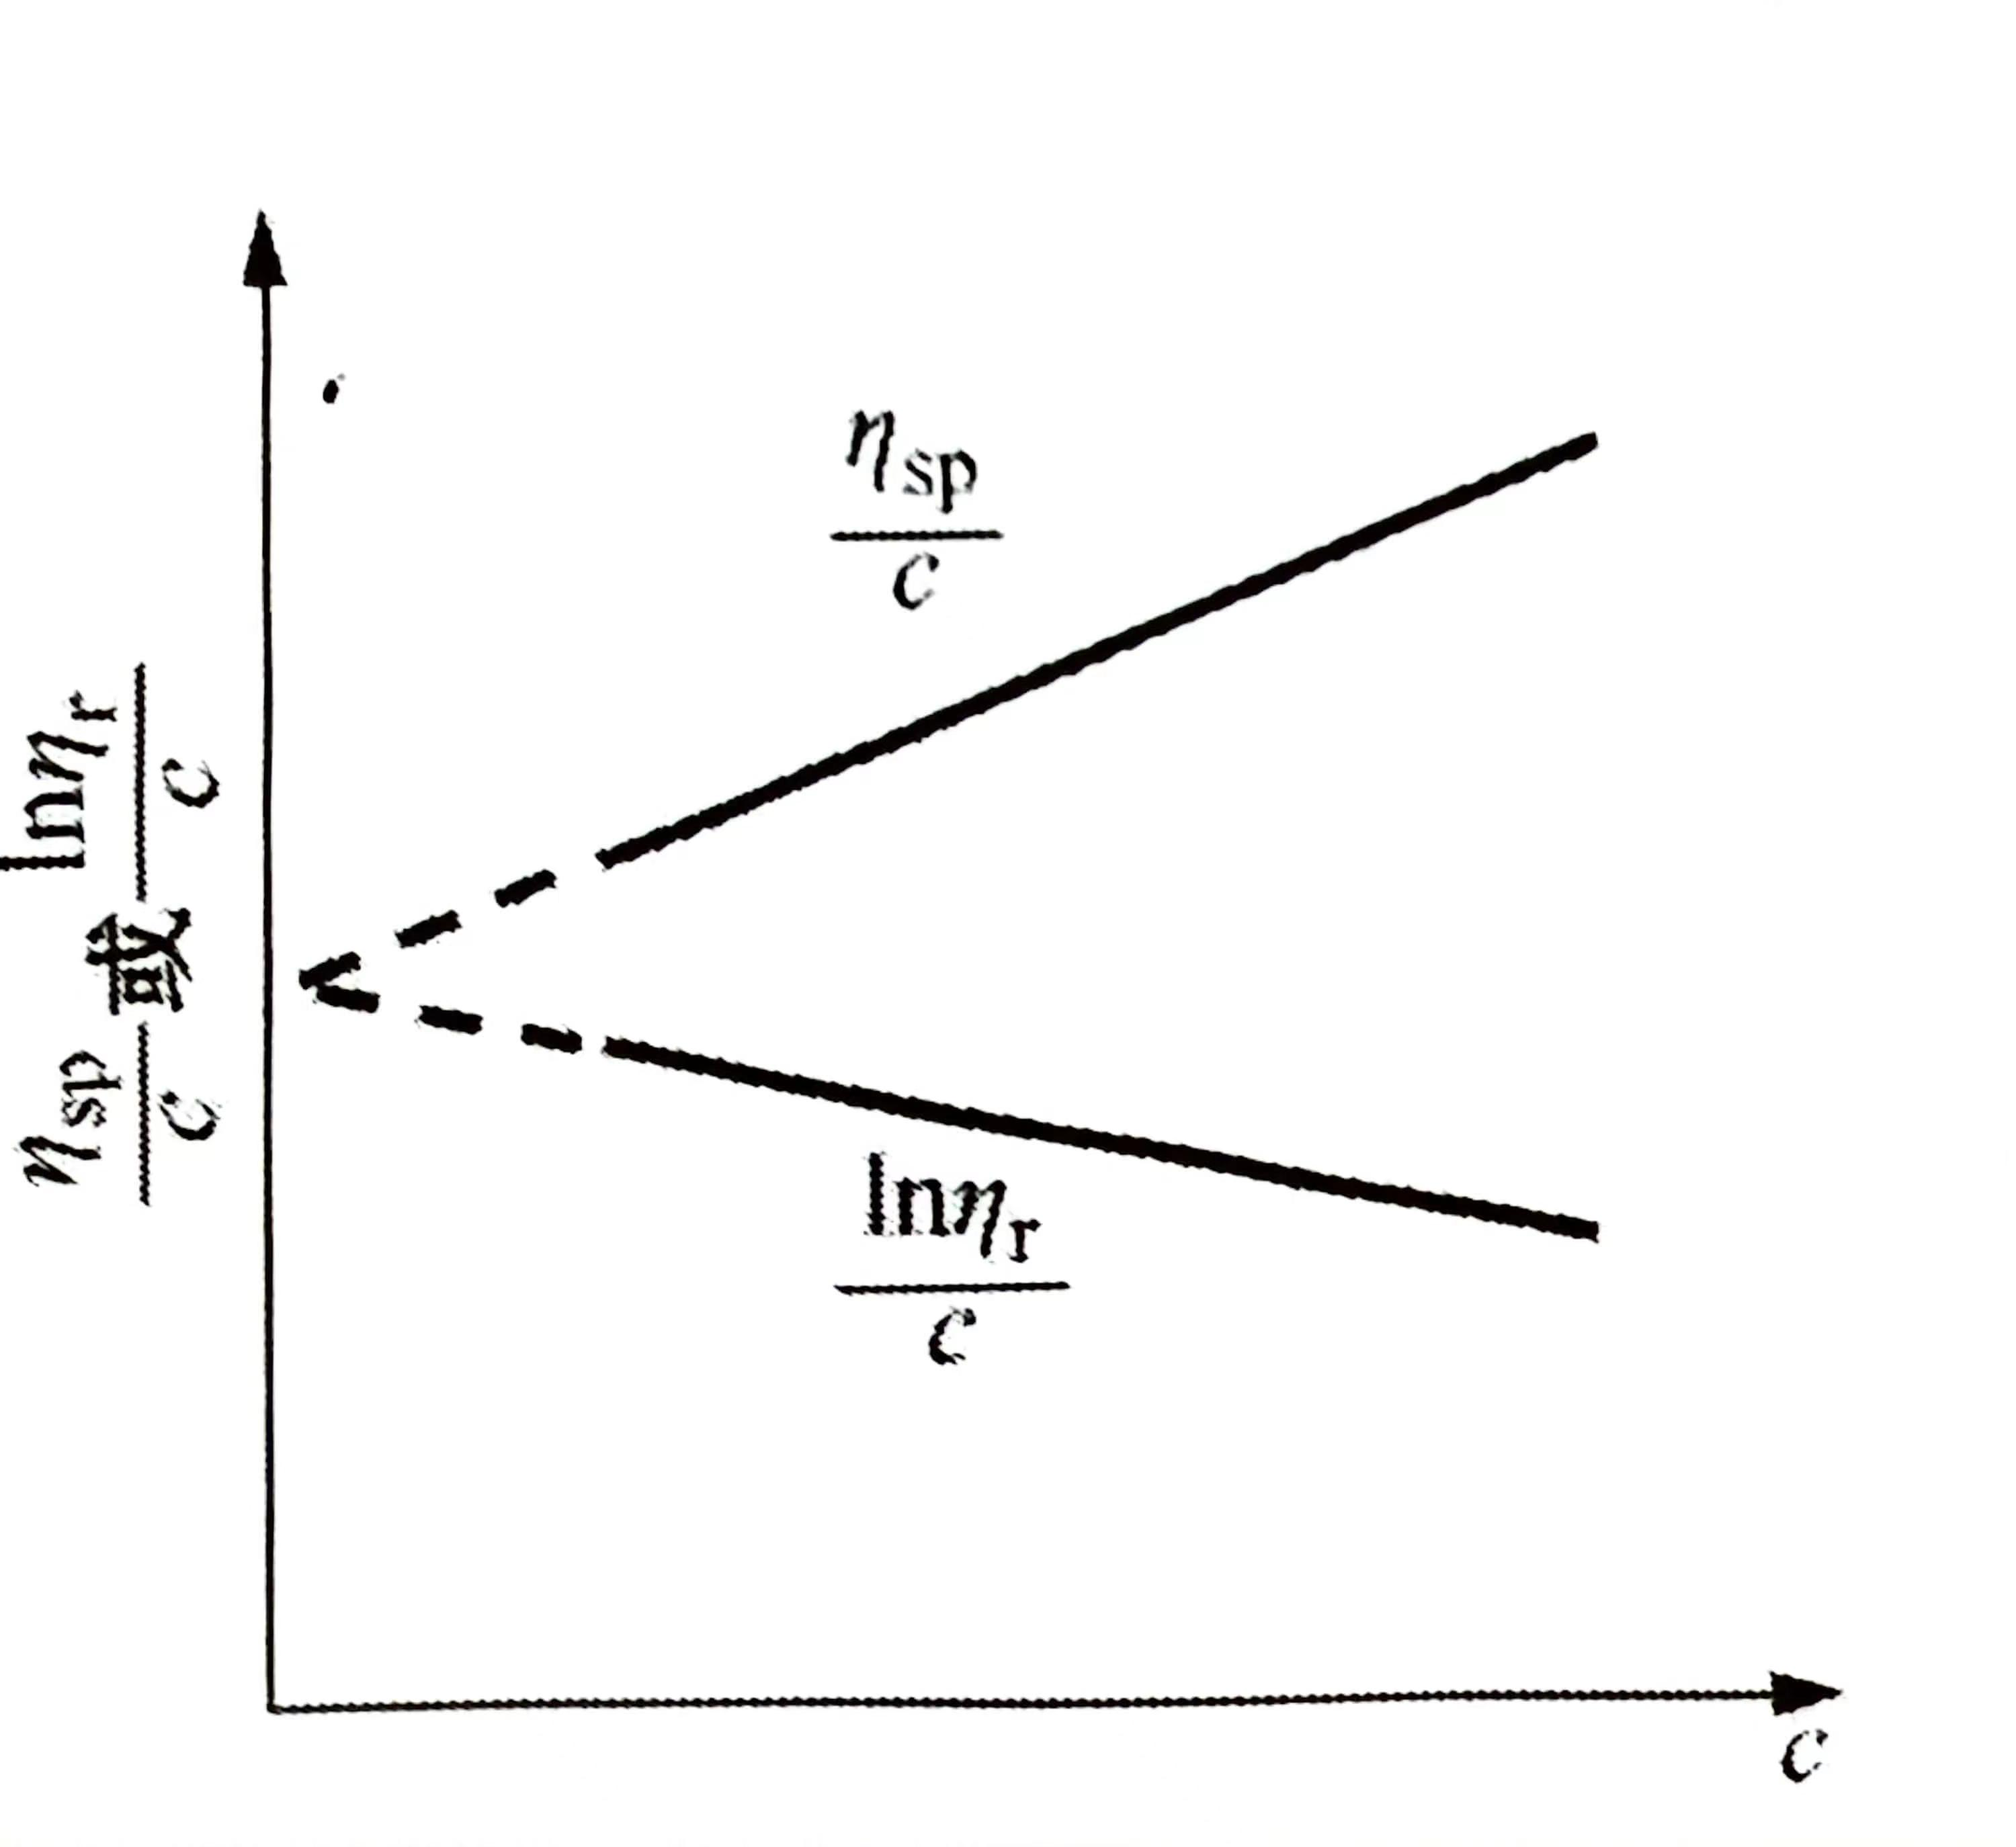
\includegraphics[width=0.5\linewidth]{WechatIMG595.jpg}
    \caption{外推法求$[\eta]$示意图}
    \label{fig:enter-label1}
\end{figure}

高聚物分子越大,则它与溶剂分子间的接触表面也就越大,摩擦越大,表现出的特性黏度越大,特性黏度与高聚物黏度平均摩尔质量间的半经验公式由马克霍温克方程给出
\begin{equation}
    [\eta] = K M^{\alpha}_\eta
\end{equation}
式中:$M^{\alpha}_\eta$为黏均相对摩尔质量;K为比例常数,$\alpha$是与分子形状有关的经验参数。K与$\alpha$的至与温度,聚合物,溶剂性质有关,在一定的相对平均摩尔质量范围内与相对平均摩尔质量大小无关。K受温度影响较大,而$\alpha$主要取决于高分子线团在某温度下某溶剂中的舒展程度。若在良性溶剂中,线团舒展,溶剂可全部或大部分穿透线团,线团上每个链段与溶液发生摩擦的机会增加,对同样大小的高聚物分子而言,摩擦增加就使$[\eta]$增大,所以$\alpha$就大,其值接近于1。相反,如在不良溶剂中,线团紧缩,使线团与溶剂发生摩擦的机会减小,使$[\eta]$亦变小,所以$\alpha$就小,在极限的情况下,已被实验结果证实$\alpha$接近于0.5,故通常说成$\alpha$介于0.5-1之间。K与$\alpha$的数值只能通过其他绝对方法进行确定。由黏度法可测得$[\eta]$,通过式(5)计算聚合物的黏均相对平均摩尔质量。
测定液体黏度的方法,主要有毛细管法-测定液体通过毛细管的流出时间;落球法-测定圆球在液体里的下落速率;转筒法-测定液体在同心轴圆柱体间相对转动的状况。在测定高分子溶液的特性黏度$[\eta]$时,以毛细管法最为方便。当液体在毛细管黏度计内因重力作用而流出时,遵守泊肃叶(Poiseuille)定律
\begin{equation}
    \frac{\eta}{\rho} = \frac{\pi hgr^4 t}{8lV} - \frac{mV}{8\pi lt}
\end{equation}

式中:$\eta$是液体的黏度;$\rho$是液体的密度;g是重力加速度;r是毛细管半径;t是流出时间;l是毛细管长度;V是时间t内流经毛细管液体的体积;h是流经毛细管液体的平均液柱高度;m是与仪器的几何形状有关的常数,通常m值大约为1.12,在$(\frac{r}{l}) \ll  1$时,取m=1。

当选用毛细管较细的黏度计测定,流出时间t>100s时,液体流动较慢,动能校正项很小,可以忽略式(6)中的第二项。

黏度的绝对值不易测定,一般都用已知黏度的液体测定毛细管常数,未知液体的黏度就可以根据在相同条件下,流过相等体积所需的时间求得。设溶液的密度与溶剂的密度近似相等,则忽略式(6)中第二项后得
\begin{equation}
    \eta _r = \frac{\eta}{\eta_0} = \frac{t}{t_0}
\end{equation}

式中:$\eta _0$和$t_0$分别为已知液体的黏度和流出时间;$\eta$和t分别为待测液体的黏度和流出时间。因此实验中,只需测定溶液和溶剂在毛细管中的流出时间就可得到$\eta_r$。

\section{仪器与试剂}
\subsection{实验仪器}
\begin{itemize}
    \item 恒温槽($\times$1)
    \item 乌氏黏度计($\times$1)
    \item 25mL容量瓶($\times$1)
    \item 洗耳球($\times$1)
    \item 5mL移液管($\times$1),10mL移液管($\times$1)
    \item 弹簧夹($\times$2),秒表($\times$1)
    \item 细乳胶管
\end{itemize}

\subsection{实验试剂}
聚乙二醇

\section{实验步骤}
\begin{enumerate}
    \item 准备工作:
    \begin{enumerate}
        \item 将恒温水浴调至$35^{\circ}C$。
        \item 配置高聚物溶液:用分析天平准确称量聚乙二醇样品约1g,在50mL烧杯中加入10mL溶剂去离子水,待固体全部溶解后定量转入25mL容量瓶中加水至刻度。
    \end{enumerate}
    \item 测定液体流出时间:

    \begin{enumerate}
\item 乌氏黏度计使用前洗净。

\item 用移液管移取15mL样品液体从A管加入黏度计的F球,在$30^{\circ}C$恒温槽内恒温5min。在C管上端口套上乳胶管并用夹子夹牢,使之不通气。B管上端口也套上乳胶管,接上洗耳球慢慢抽吸,使样品从F球经D球上升至毛细管上方的E球。当液面超过a线上小泡G的$\frac{1}{2}$处时,停止抽气,移去洗耳球,打开C管上的夹子使之通大气。此时毛细管底部液体同D管分开,G球内液面开始下降。用秒表测定液面流经a、b刻度线所需时间(即液面至a线时开始计时,液面经b线时停止计时),重复测定3次,每次流出时间相差不超过0.2-0.3s,取平均值为$t_1$。

\item  用移液管从A管加入5mL溶剂水至F球的溶液中稀释溶液,并将此稀释液用洗耳球抽洗黏度计的毛细管2-3次,使之混匀。按前述方法测定$t_2$。同样依次加10,15,15mL水,使溶液浓度为起始浓度的1/2,1/3,1/4,分别测定$t_3$,$t_4$,$t_5$。

\item 将黏度计内的溶液倒入水槽,将黏度计用去离子水冲洗干净,尤其是要仔细冲洗毛细管,用移液管移取15mL溶剂水至黏度计F球中,按上述步骤的操作测定溶剂的流出时间$t_0$。

\item 实验结束后,倒除黏度计中溶剂。
\end{enumerate}


\end{enumerate}


\section{原始数据记录}
\begin{itemize}
    \item 恒温温度:$35.00^{\circ}C$
    \item 流出时间测定:
    
    \begin{table}[htp]
    \centering
\begin{tabular}{|ll|l|l|l|l|l|l|}
\hline
\multicolumn{2}{|l|}{溶液/mL}                                                                                  & 15     & 15.00  & 15.00  & 15.00  & 15.00  & 0.00  \\ \hline
\multicolumn{2}{|l|}{累计加入溶剂/mL}                                                                              & 0      & 5      & 15     & 30     & 45     & 0     \\ \hline
\multicolumn{2}{|l|}{相对浓度c}                                                                                  & 1      & 0.75   & 0.5    & 1/3    & 0.25   & 0     \\ \hline
\multicolumn{1}{|l|}{\multirow{4}{*}{\begin{tabular}[c]{@{}l@{}}溶液\\ 流出\\ 时间\\ \\ \\ \end{tabular}}} & t/s   & 316.24 & 240.27 & 174.27 & 141.04 & 126.15 & 86.13 \\ \cline{2-8} 
\multicolumn{1}{|l|}{}                                                                               & t/s   & 315.56 & 240.06 & 173.88 & 141.24 & 126.24 & 87.25 \\ \cline{2-8} 
\multicolumn{1}{|l|}{}                                                                               & t/s   & 315.94 & 240.15 & 174.20 & 141.31 & 125.59 & 86.44 \\ \cline{2-8} 
\multicolumn{1}{|l|}{}                                                                               & 平均t/s & 315.91 & 240.16 & 174.12 & 141.20 & 125.99 & 86.61 \\ \hline
\end{tabular}
\end{table}

\end{itemize}



\section{数据处理}
\subsection{数据处理与归纳}
\begin{table}[htp]
\centering
\begin{tabular}{|ll|l|l|l|l|l|l|}
\hline
\multicolumn{2}{|l|}{溶液/mL}                                                                                  & 15     & 15.00  & 15.00  & 15.00  & 15.00  & 0.00  \\ \hline
\multicolumn{2}{|l|}{累计加入溶剂/mL}                                                                              & 0      & 5      & 15     & 30     & 45     & 0     \\ \hline
\multicolumn{2}{|l|}{相对浓度c}                                                                                  & 1      & 0.75   & 0.5    & 1/3    & 0.25   & 0     \\ \hline
\multicolumn{1}{|l|}{\multirow{4}{*}{\begin{tabular}[c]{@{}l@{}}溶液\\ 流出\\ 时间\\ \\ \\ \end{tabular}}} & t/s   & 316.24 & 240.27 & 174.27 & 141.04 & 126.15 & 86.13 \\ \cline{2-8} 
\multicolumn{1}{|l|}{}                                                                               & t/s   & 315.56 & 240.06 & 173.88 & 141.24 & 126.24 & 87.25 \\ \cline{2-8} 
\multicolumn{1}{|l|}{}                                                                               & t/s   & 315.94 & 240.15 & 174.20 & 141.31 & 125.59 & 86.44 \\ \cline{2-8} 
\multicolumn{1}{|l|}{}                                                                               & 平均t/s & 315.91 & 240.16 & 174.12 & 141.20 & 125.99 & 86.61 \\ \hline
\multicolumn{2}{|l|}{$\eta _r$}                                                                                     & 3.6476 & 2.7730 & 2.0104 & 1.6303 & 2.4547 & /     \\ \hline
\multicolumn{2}{|l|}{ln$\eta _r$r}                                                                                   & 1.2941 & 1.0199 & 0.6983 & 0.4888 & 0.3748 & /     \\ \hline
\multicolumn{2}{|l|}{ln$\eta _r$/c}                                                                                 & 1.2941 & 1.3599 & 1.3967 & 1.4663 & 1.4993 & /     \\ \hline
\multicolumn{2}{|l|}{$\eta _{sp}$}                                                                                    & 2.6476 & 1.7730 & 1.0104 & 0.6303 & 0.4547 & /     \\ \hline
\multicolumn{2}{|l|}{$\eta _{sp}$/c}                                                                                  & 2.6476 & 2.3640 & 2.0209 & 1.8910 & 1.8189 & /     \\ \hline
\end{tabular}
\end{table}



\subsection{拟合与可视化}
具体数据处理过程和结果见附页

\begin{figure}[H]
	\centering
	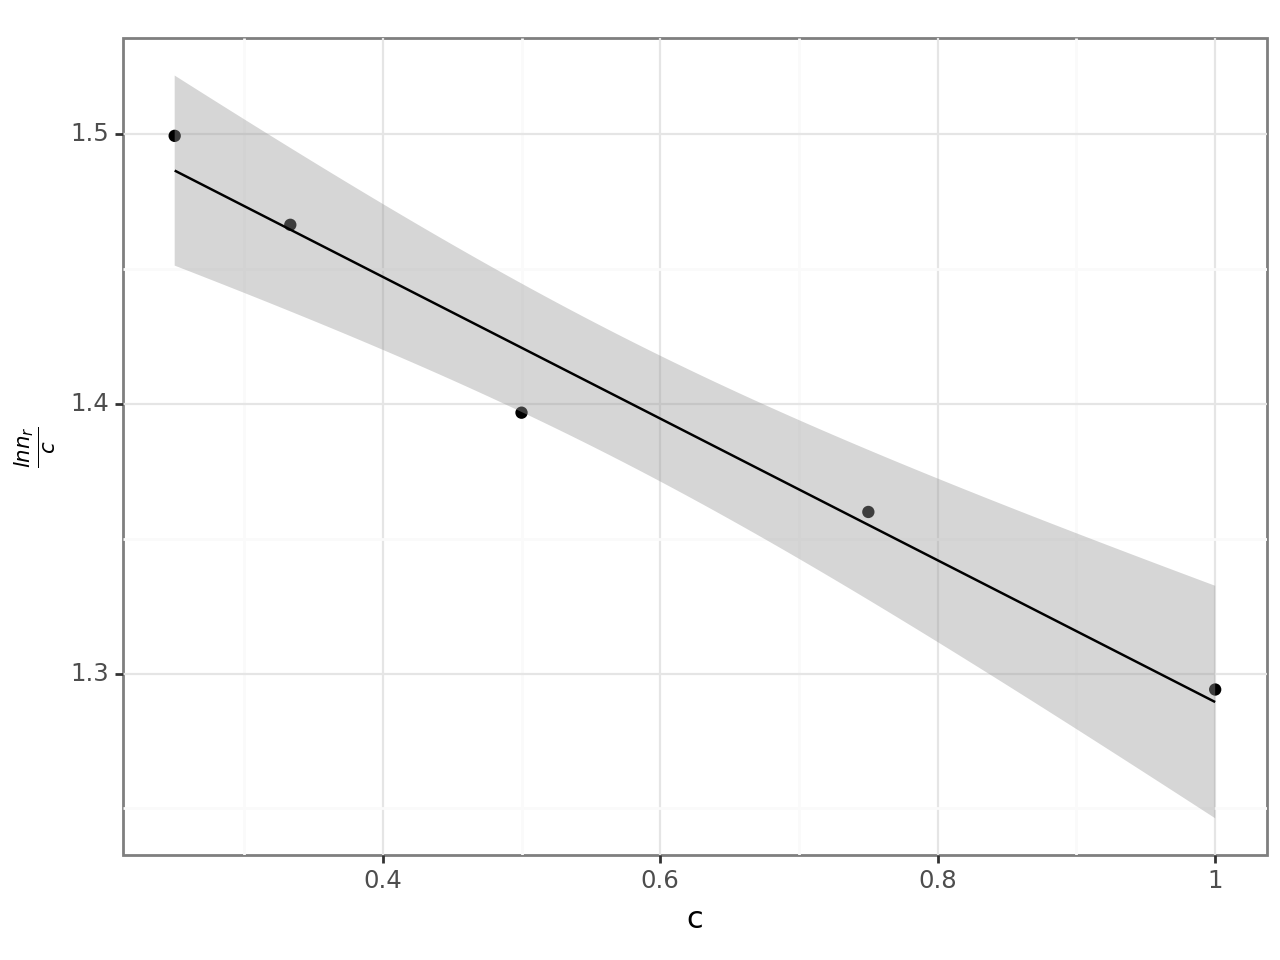
\includegraphics[width=0.7\linewidth]{fig1.png}
	\caption{ln$\eta _{sp}$/c对相对浓度c线性拟合图}
	\label{fig:enter-label}
\end{figure}
\begin{figure}[H]
	\centering
	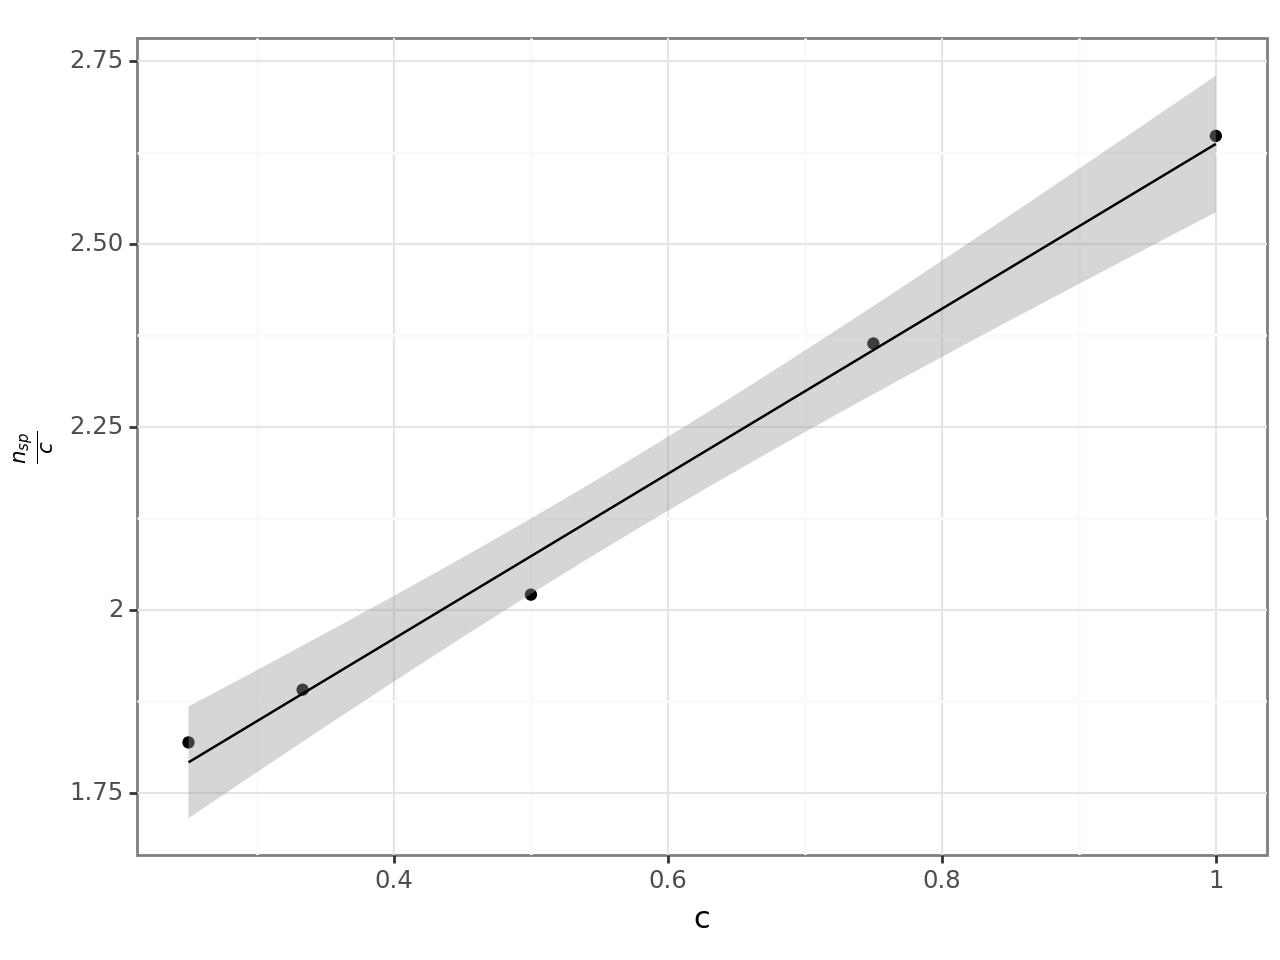
\includegraphics[width=0.7\linewidth]{fig2.png}
	\caption{$\eta _{sp}$/c对相对浓度c线性拟合图}
	\label{fig:enter-label}
\end{figure}


\begin{figure}[H]
    \centering
    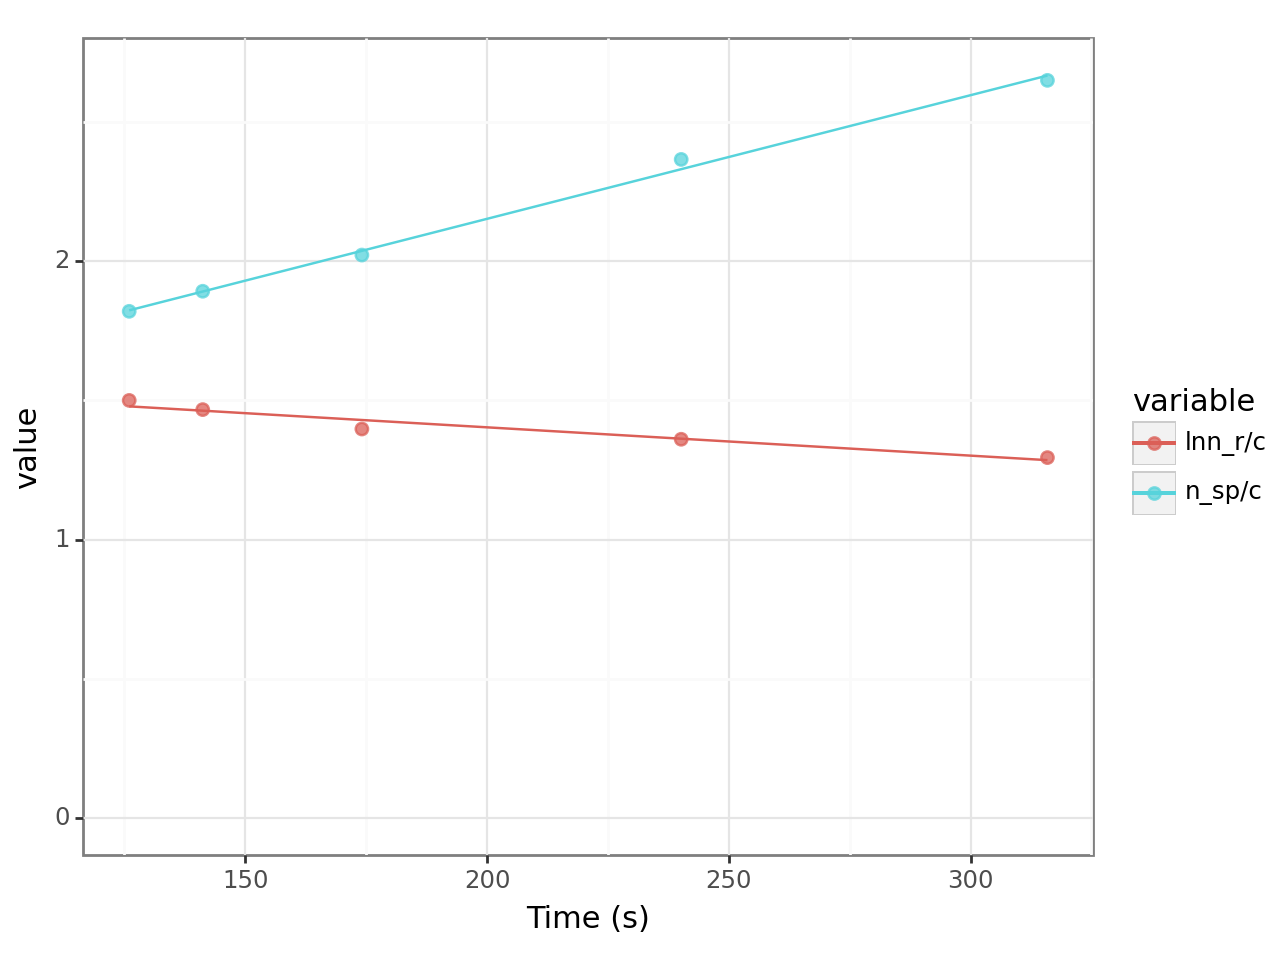
\includegraphics[width=0.7\linewidth]{fig3.png}
    \caption{外推法求特性黏度示意图}
    \label{fig:enter-label}
\end{figure}


ln$\eta _{sp}$/c对相对浓度c图像截距为1.5521,Adj. R-squared为0.990, 说明线性模型拟合结果非常好;$\eta _{sp}$/c对相对浓度c截距为1.5101,Adj. R-squared为0.921,线性关系强烈,但是两者截距不一致,故以$\eta _{sp}$/c对相对浓度c图像截距为基准,得截距A=1.5101.故特性黏度\begin{equation}
    [\eta] = \frac{A}{c_0} = \frac{1.5101}{20kg\cdot m^{-3}} = 0.075505 m^3\cdot kg^{-1}
\end{equation}

又由式(5)可得聚乙二醇的黏均相对摩尔质量
\begin{equation}
     \overline{M_\eta} = \sqrt[\alpha]{\frac{[\eta]}{K}} = \sqrt[0.82]{\frac{0.075505}{6.4\times 10^{-6}}} = 9.238\times 10^4
\end{equation}

\section{结果分析与讨论}
\subsection{结果分析}
在本实验中,我们所测定的聚乙二醇的黏均相对摩尔质量为 $9.238 \times 10^4$。根据已有的文献资料,聚乙二醇在 $35^\circ C$ 下的黏均相对摩尔质量应介于 $3 \times 10^4$ 与 $7 \times 10^4$ 之间。因此,实验结果与文献值相比位于合理范围之内,显示实验结果具有一定的可靠性。然而,通过对拟合模型的分析,我们得到的调整后的 R 方(Adj. R-squared)分别为 0.921 和 0.990,这表明虽然模型拟合程度良好,但实验数据与模型仍存在一定的偏差。此外,记录溶液流出时间的数据显示,有多组数据的流出时间差异超过了 0.3 秒,这暗示了潜在的实验误差。为了深入探讨实验误差的可能来源,以下是几个潜在的误差因素:
\begin{itemize}
    \item 温度的影响对于高分子溶液的粘度具有显著影响。\cite{1}为保证实验结果的准确性,实验应在恒温条件下进行,且温度的波动范围应严格控制在 $0.05^\circ C$ 以内。本实验中由于实验操作在 $30^\circ C$ 下进行了较长时间,随后的温度改变可能未能等待恒温水槽达到稳定状态便开始实验,这可能导致了实验误差。
    \item 较稀和较高浓度的溶液也会导致实验误差\cite{2},这是由于当浓度较高和较稀的时候,操作和仪器带来的误差转化为相对误差就会变得非常大,带来误差。
    \item 实验操作过程中,每次更换溶液后,必须对黏度计的B管进行彻底的清洗和排气。由于本实验对精度要求较高,先前溶液的残留以及黏度计内部气泡的排除显得尤为关键,这些因素可能会改变溶液的实际浓度,并影响流出时间的测定。但是,由于实验条件的限制,这类误差很难完全消除。
    \item 溶液中不可以存在微粒杂质,由于毛细管半径非常细,如果存在这类杂质,那么就会导致局部堵塞现象而影响液体流出时间\cite{3}。粘度计在保存和清洗过程中都应该防止尘埃进入。
    \item 本实验中使用的聚乙二醇溶液密度为20$kg\cdot m^{-3}$,实验结果中两条拟合曲线未相交于y轴上,以$\eta _{sp}$/c对相对浓度c图像为参照,求得截距。而根据《黏度法测聚乙二醇相对分子质量的几种情况讨论》\cite{1},样品的质量浓度在24g/L与32g之间时,两条拟合直线可以相交于纵坐标轴。在浓度范围选择不当的情况下,黏度计的构造因素以及其他非系统误差(如黏度计每次浓度
切换时毛细管的清洗,黏度计垂直程度等)对实验结果的影响就能表现出来,而拟合图形对实验数据非
常敏感,测量数据中往往小数点后一位的变化就会改变图形趋势,造成难以分析的情况。因此,改变聚乙二醇溶液浓度有助于使得测量精度更高。
\end{itemize}

\subsection{总结与改进}
在本次实验中,我们采用黏度法来测定水溶性高聚物——聚乙二醇的相对平均摩尔质量。实验的核心是掌握乌贝路德黏度计的使用和理解黏度法的原理。通过测量不同浓度下聚乙二醇溶液的黏度与纯溶剂的黏度,并计算增比黏度 $\eta_{sp}$,我们得以评估高聚物的摩擦特性,进而推算出聚乙二醇的特性黏度 $[\eta]$。

在实验流程上,我们首先准备了一系列不同浓度的聚乙二醇溶液,并确保了实验条件的恒定,特别是温度的控制,因为黏度与温度有显著的依赖关系。利用乌贝路德黏度计测定了每个溶液的流动时间,再转换为相对黏度 $\eta_{r}$。在数据处理过程中,我们对 $\eta_{sp}/c$ 和 $\ln{\eta_{r}/c}$ 与溶液浓度 $c$ 进行了图形外推,以便在无限稀释情况下,确定聚乙二醇的特性黏度 $[\eta]$。

通过实验,我们发现聚乙二醇的特性黏度与其摩尔质量成正比,且马克霍温克方程对我们的实验结果具有良好的适应性。实验结果表明,随着聚乙二醇分子量的增加,其与溶剂分子间的摩擦增加,导致特性黏度增大。这与理论预期相符合,证实了我们的实验操作与数据处理是正确的。

总体而言,本次实验不仅让我们深入理解了黏度法的原理和操作技巧,还提高了我们处理实验数据和解析实验结果的能力。我们也意识到实验中可能存在的系统误差,并在分析与讨论部分提出了相应的改进措施。未来,我们可以通过进一步优化实验条件和方法,来提高实验的精度和可靠性。

而针对上一部分中分析的实验误差来源,我们提出以下改进措施和建议:

\begin{enumerate}
	\item \textbf{温度控制}:应使用高精度温度控制装置,并确保实验过程中温度稳定性优于 $0.05^\circ C$。此外,应在每次测量前等待足够时间,以确保温度控制系统达到平衡状态。
	
	\item \textbf{浓度的适宜性}:优化溶液的浓度范围,通过预实验确定最佳的浓度,以减小操作和仪器误差对最终结果的影响。
	
	\item \textbf{仪器清洗与排气}:改进黏度计的B管清洗和排气步骤,可能的话使用自动化装置以减少人为误差。确保每次测量前B管内无气泡和残留溶液。
	
	\item \textbf{杂质控制}:在实验前彻底清洗所有实验器材,并在实验过程中避免尘埃和杂质的污染。对于黏度计,可以考虑使用过滤器或其他过滤设备以去除微粒杂质。
	
	\item \textbf{测量方法的改进}:探索使用其他稳定性更强、精度更高的测量设备或方法,比如差示扫描量热仪(DSC)或动态光散射(DLS)等,以获得更为准确可靠的数据。
	
	\item \textbf{数据处理}:增强数据处理的严谨性,增加数据的测量数,采用更高级的统计分析方法,以识别和剔除异常数据点(例如计算p-value,或绘制置信区间),从而提高实验结果的准确度和重复性。
\end{enumerate}

\section{思考题}

\subsection{乌氏黏度计中的支管C有什么作用?除去支管C,是否仍可测黏度?}

支管C(放空管)的功能是确保毛细管两端压力的平衡,并且允许空气自由流动以避免液体流动时产生的真空吸引效应。这有助于防止液体中产生湍流,确保液体以层流的形式通过毛细管,从而提高测量的精确性。尽管没有C管也可以进行黏度测量,但是测量的准确性和重复性将显著下降,因为去除C管后,毛细管两端将不再保持压力平衡,且容易引入气泡干扰。

\subsection{乌氏黏度计的毛细管太粗或太细各有什么缺点?}

毛细管的内径对于黏度测量至关重要。如果毛细管太粗,将导致液体流动速度过快,使得测量时间缩短而难以准确测量,并且可能需要计算动能校正项,从而影响测量的准确性。相反,如果毛细管太细,液体流动速度会变慢,可能导致与管壁的摩擦增加,并且实验时间会不必要地延长。此外,细管更可能堵塞,维护和清洁也更加困难。

\subsection{利用黏度法测定高聚物相对摩尔质量的局限性有哪些?}

\begin{itemize}
	\item 黏度法的适用性有限,它最适合用于测量一定范围分子量的高聚物,对于分子量过大或过小的高聚物,测定的准确性会降低。
	\item 该方法基于经验公式,如果样品的分子量分布不均匀,这些公式可能无法准确描述所有分子的黏度行为。
	\item 实验条件对黏度测量结果有显著影响,包括溶剂选择和溶液浓度等,这些都需要严格控制以确保结果的可靠性。
\end{itemize}

\subsection{特性黏度$[\eta]$就是溶液无限稀释时的比浓黏度,它和纯溶剂的黏度是否一样?为什么要用特性黏度求高聚物的相对摩尔质量?}

特性黏度$[\eta]$是指在无限稀释条件下溶液的比浓黏度。它不同于纯溶剂的黏度,因为特性黏度考虑了溶液中高聚物分子所增加的黏度。在无限稀释状态下,高聚物分子相互作用可以忽略,因此特性黏度主要反映的是高聚物分子与溶剂分子之间的相互作用。由于特性黏度是高聚物摩尔质量的一个固有属性,它可以用来计算高聚物的相对摩尔质量,提供了一种测量这一重要物理参数的方法。



%%----------- 参考文献 -------------------%%
%在reference.bib文件中填写参考文献,此处自动生成

\reference


\end{document}